\section{评测结果}

\subsection{程序清单}

\begin{enumerate}
\item sim.cc:传统方法仿真脚本
\item tcp\_base.py:Deep Q-learning算法模型
\item tcp\_newreno.py:newreno算法实现
\item tcp-rl-env.cc:网络环境在强化学习当中的环境构建
\item tcp-rl.cc:强化学习环境构建
\item test\_tcp.py:强化学习运行脚本
\end{enumerate}

\subsection{实验结果}

\begin{figure}[htbp]
	\centering
	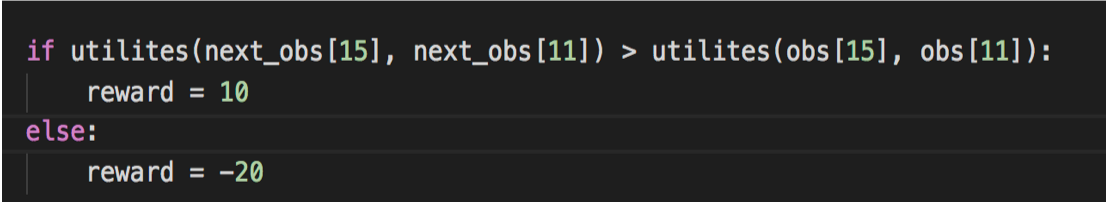
\includegraphics[width=0.8\linewidth]{figure/figure7.png}
	\caption{改进reward}
	\label{figure7}
	\centering
	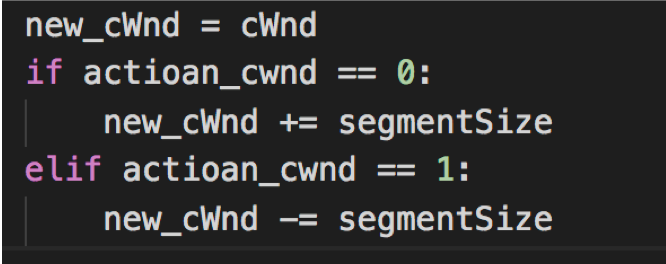
\includegraphics[width=0.6\linewidth]{figure/figure8.png}
	\caption{改进action}
	\label{figure8}
\end{figure}

\begin{figure}[htbp]
\centering
\begin{minipage}[t]{0.48\textwidth}
\centering
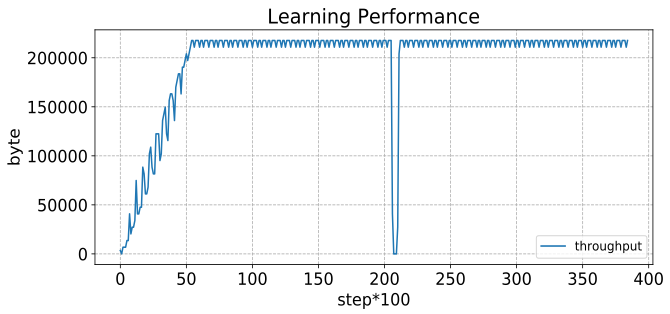
\includegraphics[width=6cm]{figure/figure9.png}
\caption{throughput}
\end{minipage}
\begin{minipage}[t]{0.48\textwidth}
\centering
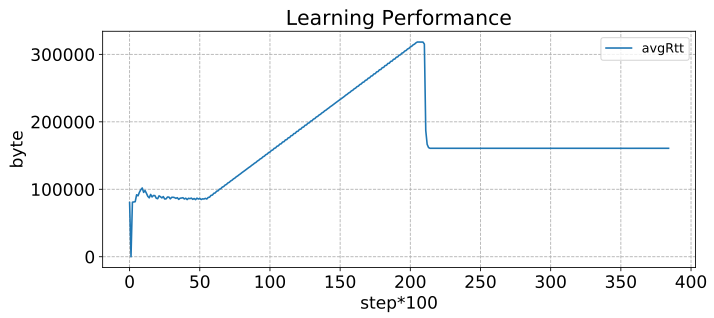
\includegraphics[width=6cm]{figure/figure10.png}
\caption{avgRTT}
\end{minipage}
\centering
\begin{minipage}[t]{0.48\textwidth}
\centering
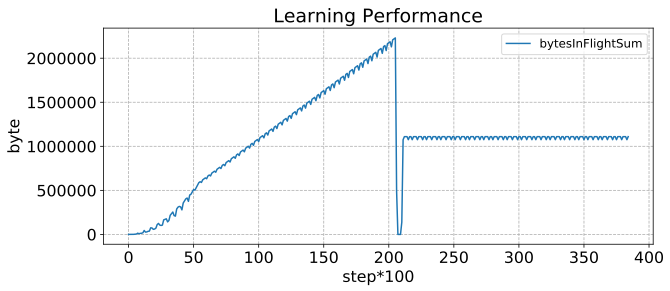
\includegraphics[width=6cm]{figure/figure11.png}
\caption{bytesInFlightSum}
\end{minipage}
\begin{minipage}[t]{0.48\textwidth}
\centering
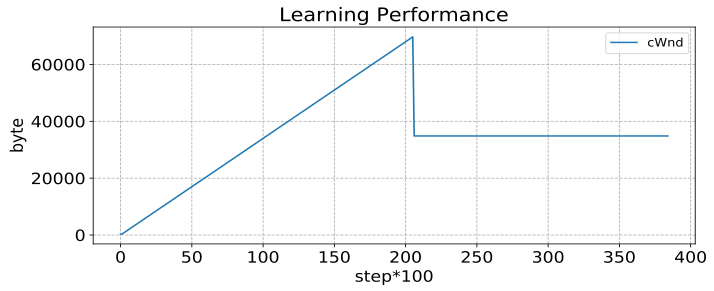
\includegraphics[width=6cm]{figure/figure12.png}
\caption{CWND}
\end{minipage}
\end{figure}

改进后,1个step的平均运行速度为0.007s,收敛速度也超过了论文水平。由此可见,强化学习方法在计算机网络领域作用是能起到作用的。